
%Introduce the NOvA detectors and give big picture overview
The NOvA experiment (NuMI Off-axis $\nu_e$ Appearance) consists of two
detectors which measure the neutrino composition of the NuMI
(Neutrinos at the Main Injector). The
300~ton near detector is on site at Fermilab and is located 1.015~km
from the NuMI
target hall. The 14~kiloton far detector is located 810km from the
NuMI target hall. Both detectors are placed off-axis from the centre
of the NuMI beam by 14.6~mrads.

The original design of the NOvA experiment is laid out in the
technical design report (TDR) \cite{TDR}. The constructed experiment
differs only slightly with the design laid out in the TDR. The details
of the constructed experiment, including the neutrino beam source and
the two detectors, are discussed in the following chapter.


\section{The NuMI Beam}

The NOvA experiment's neutrino source is provided by the Neutrinos at
the Main Injector (NuMI) beam at Fermilab. The following section
describes the process by which the NuMI muon neutrino beam is created.

%Paragraph in notes form. Revisit!
An instructive diagram of the NuMI beam is presented in
Figure~\ref{fig:NuMI}.
The Main Injector accepts six batches, each spanning 10~$\mu$sec, of
protons at a time and accelerates the protons up to 120~GeV. The
accelerated protons are directed to collide with a 95cm long graphite
target. The collision protons with the carbon atoms of the target
produce a plethora of mesons (mostly pions and kaons). The charged
mesons are focused into a beam by two magnetic focussing horns. The
focussing horns are run in Forward Horn Current (FHC) or Reverse Horn
Current (RHC)
mode to select positively or negatively charged mesons
respectively, leading to a neutrino or an anti-neutrino beam respectively. 

The focussed beam of charged mesons then travels through a 675~m long
evacuated decay pipe. Along this length of pipe the mesons decay to charged
leptons and neutrinos. The decay pipe is followed by hadron and muon
monitors and about 240m of rock. The rock absorbs the remaining charged
particles in the beam before reaching the near detector.




after main description talk about the beam upgrades: slip-stacking
and power. water cooling 



% NuMI beam figure
%\begin{figure}[!ht]
\begin{figure}
  \centering
  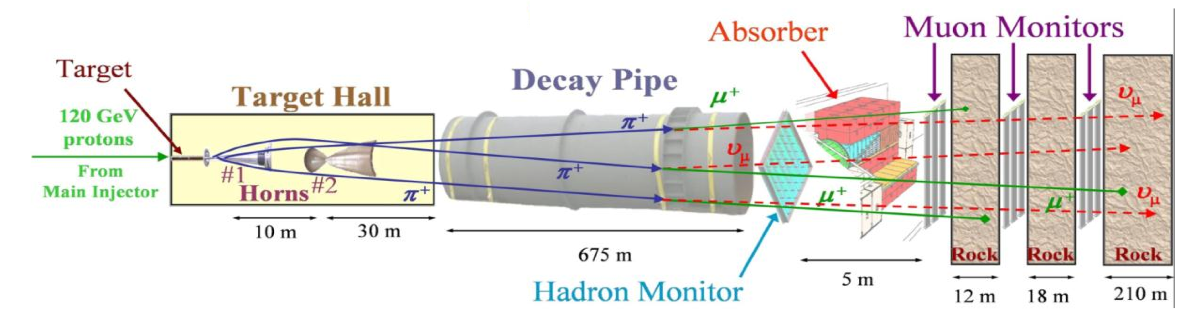
\includegraphics[width=1\textwidth]{../../img/beam/beam_diagram.png}
  \caption{A diagram showing the layout of the NuMI beam.}
  \label{fig:NuMI}
\end{figure}


\subsection{Off-axis Detectors}

The NOvA detectors are both placed 14~mrads off the axis of the NuMI
beam.
The reasons for placing the detector will be described
in more detail in the following paragraphs. 
% Placing the detectors off-axis has the advantages of increasing
% the neutrino flux at NOvA's oscillation maximum and reducing
% backgrounds.

The decay used to produce a neutrino beam is a two body decay, where a
pion (or kaon) decays to a neutrino and a muon. The two body decay 
occurs isotropically in the parent particles rest frame. 
In the lab frame the parent particle is not at rest when decaying. For
pion and kaon decay this boosts the neutrinos into a cone in the
direction of the parent particle.
For small angles, the flux and energy of neutrinos produced by pion
decay ($\pi \rightarrow \nu_{\mu} + \mu$) are given by:

\begin{equation}
\Phi = \left( \dfrac{2\gamma}{1+\gamma^2 \theta^2} \right)^2 \dfrac{A}{4\pi z^2}
\label{eqn:NuPiFlux}
\end{equation}

\begin{equation}
E_{\nu} = \dfrac{0.43E_{\pi}}{1+\gamma^2\theta^2},
\label{eqn:NuPiEnrgy}
\end{equation}

where $E_{\pi}$ is the energy of the parent pion, $m_{\pi}$ the mass of the
parent pion, $\theta$ the angle between the pion and neutrino
directions and $\gamma = E_{\pi}/m_{\pi}$.

Equations~\ref{eqn:NuPiFlux}~and~\ref{eqn:NuPiEnrgy} and are shown as 
functions of neutrino energy and off-axis angle in
Figure~\ref{fig:NuPiFlux}.
Figure~\ref{fig:NuESpectra_MEAndLE} shows the number of neutrino
events as a function of the
charged current $\nu_{\mu}$ energy for the Low (left plot) and
Medium (right plot) Energy Tune for various off-axis angles. 

For the Medium Energy Tune, figure~\ref{fig:NuPiFluxb} shows that at
14~mrad the neutrino energy
does not have a strong dependence on the parent pion energy.
In addition, figure~\ref{fig:NuESpectra_MEAndLE_b} shows that at
14~mrad the Medium
Energy Tune produces a narrow energy neutrino beam with approximately
4 times more neutrinos at 2GeV than the on-axis scenario. This peak at
2~GeV is well matched to the expected energy of the oscillation
maximum for electron neutrino appearance.





\begin{figure}
  \centering
  \begin{subfigure}[b]{0.45\textwidth}
  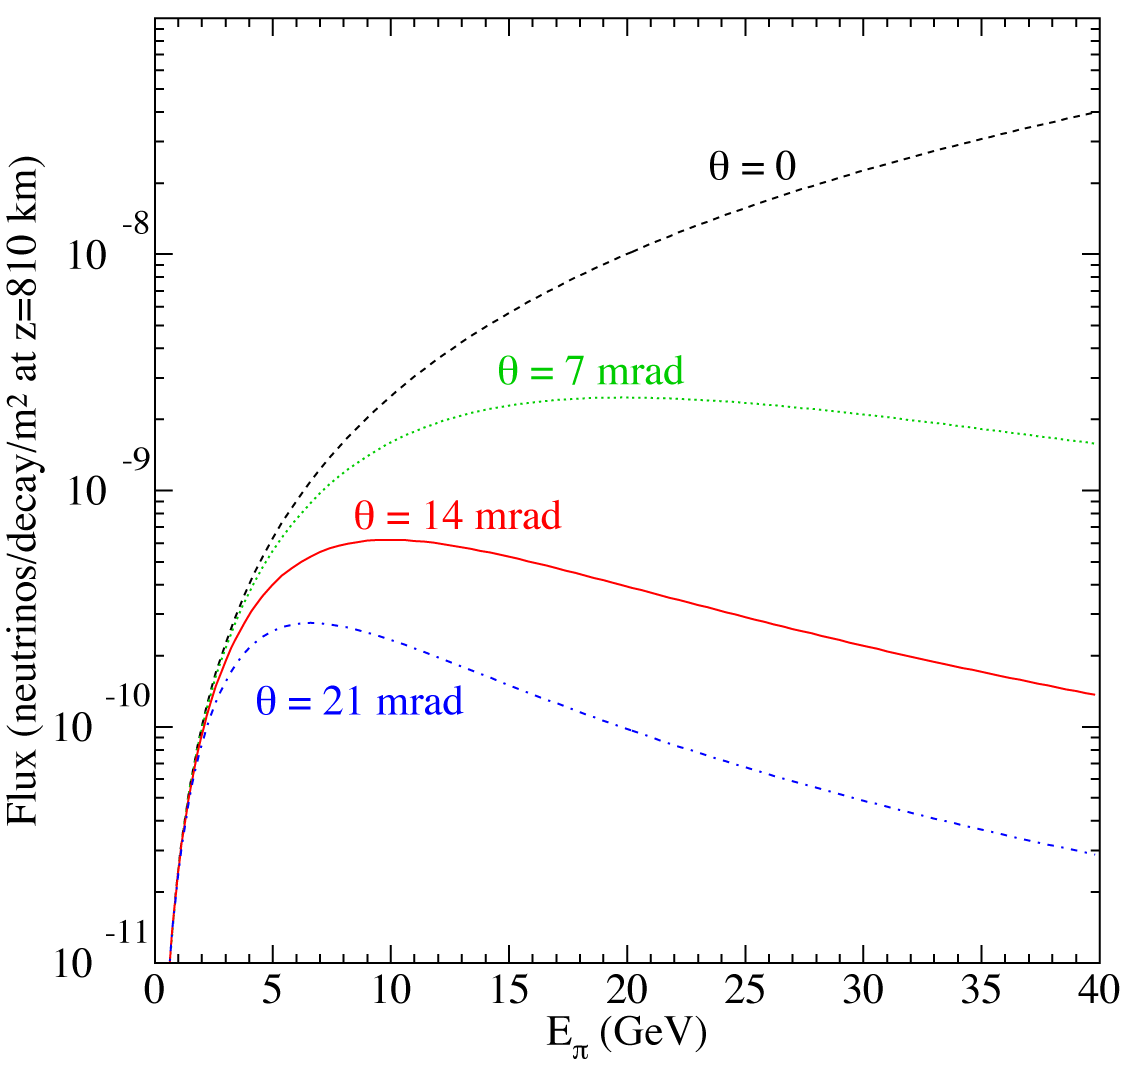
\includegraphics[width=\textwidth]{../../img/baird/beam/020-flux.png}
  \caption{Neutrino flux vs. pion energy. }
  \label{fig:NuPiFluxa}
  \end{subfigure}
  \hfill
  \begin{subfigure}[b]{0.45\textwidth}
  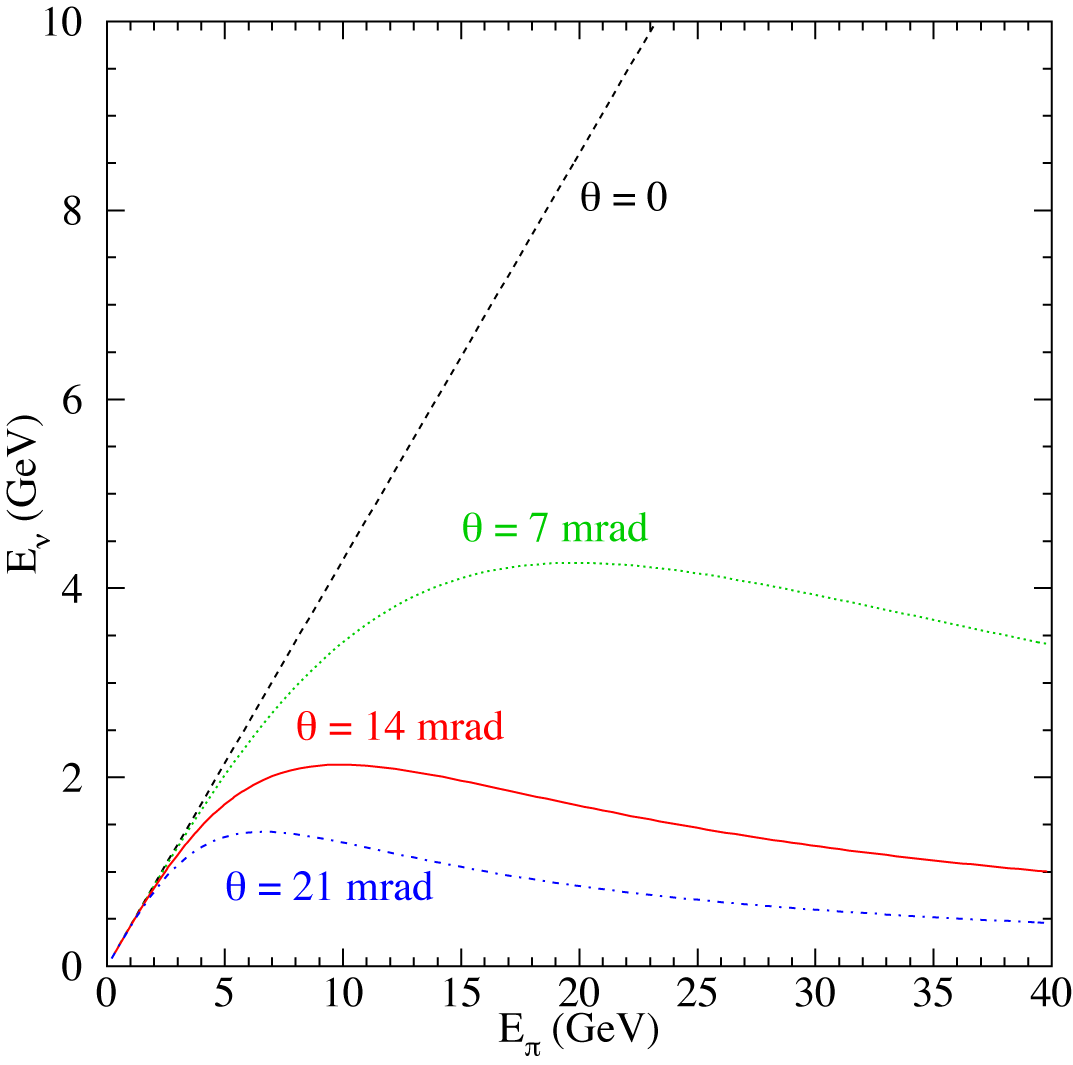
\includegraphics[width=\textwidth]{../../img/baird/beam/030-epi2enu.png}
  \caption{Neutrino energy vs. pion energy.}
  \label{fig:NuPiFluxb}
  \end{subfigure}
  \caption{The above distributions are as viewed from a site located
    800km from the NuMI target and off-axis by an angle $\theta$.}
  \label{fig:NuPiFlux}
\end{figure}



\begin{figure}
  \centering
  \begin{subfigure}[b]{0.45\textwidth}
    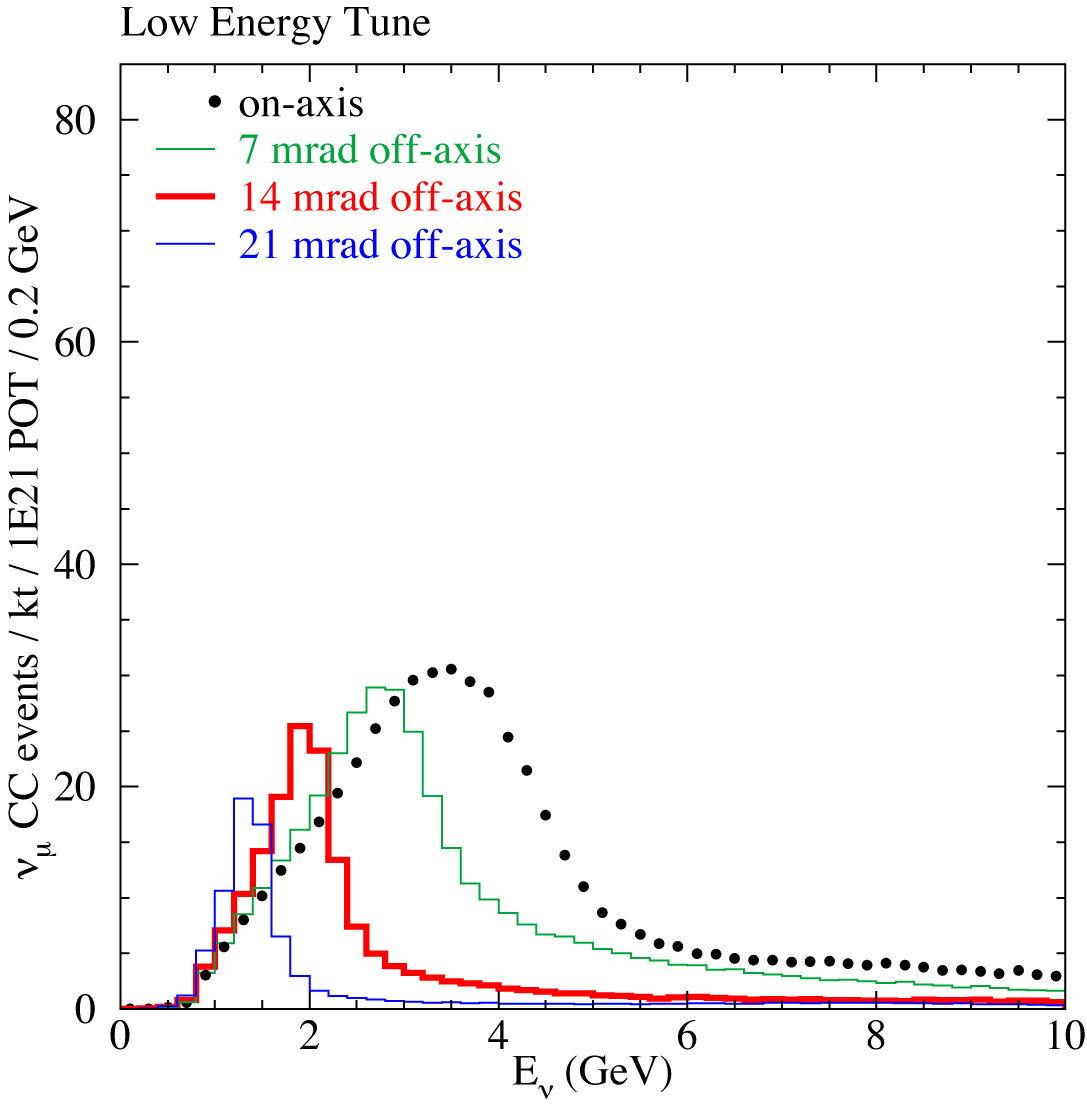
\includegraphics[width=\textwidth]{../../img/baird/beam/040-le-spectra.png}
    \caption{Low energy NuMI tune neutrino energy. \\ }
    \label{fig:NuESpectra_MEAndLE_a}
  \end{subfigure}
  \hfill
  \begin{subfigure}[b]{0.45\textwidth}
    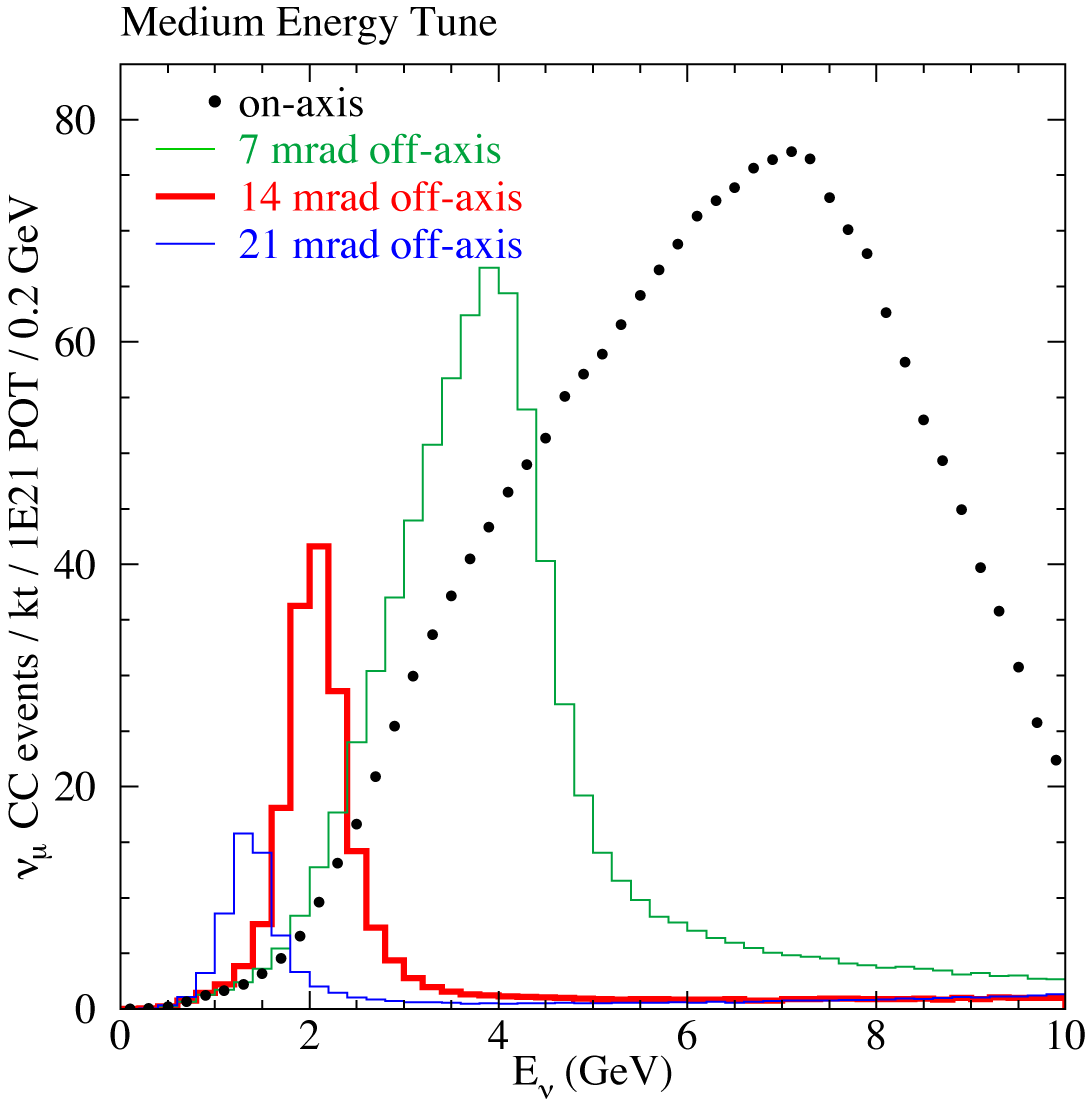
\includegraphics[width=\textwidth]{../../img/baird/beam/050-me-spectra.png}
    \caption{Medium energy NuMI tune neutrino energy.}
    \label{fig:NuESpectra_MEAndLE_b}
  \end{subfigure}
  \caption{Charged current $\nu_{\mu}$ event rates vs. neutrino
    energy in the absense of oscillations. The distributions are found
  for a detector which is 800~km from the NuMI target and for various
  off-axis angles.}
  \label{fig:NuESpectra_MEAndLE}
\end{figure}




\subsection{Horn Position}


\section{The NOvA Detectors}

The NOvA experiment uses a near and far detector to measure neutrino
oscillations. The near detector is used to measure the unoscillated
neutrino energy spectrum and the electron neutrino component of the
beam. The unoscillated neutrino energy spectrum measured by the near
detector is extrapolated to the far detector (\textcolor{red}{need to
  discuss further in a future chapter}). The far detectors purpose is
to measure the energy spectrum of the beam neutrinos for comparison
with the extropalted near detector energy spectrum.

The NOvA experiment aims to perform both $\nu{\mu}$ disappearance and
$nu_e$ appearance measurements. The
detectors are designed to distinguish electron and muon neutrino
charged current events from backgrounds. 


\subsection{Detector Construction}

%include all information common among both detectors.
The near and far NOvA detectors are almost functionally
identical. Besides
the different masses there are a few physical
differences. The near detector has a so called ``muon catcher'', has a
higher rate of readout and uses slighlty different APDs. The
construction common among both detectors will be discussed in the
following section. The details specific to the far and near detectors
will be discussed in Subsections~\ref{sec:fardet} and
\ref{sec:neardet} respectively.

%build the detector starting with the cell:
The NOvA detectors are constructed using extruded PVC tubes. Each PVC
tube is called a cell and is filled with liquid scintillator and a
Wave Length Shifting (WLS) fibre (see Figure~\ref{fig:cell}). 
18 cells are glued together side by side to form a module (see
Figure~\ref{fig:module}). Modules are then glued together, again side
by side,
to form a plane. The planes layered with alternating orthogonal
orientations, such that the orientation of the cells making up the
plain alternate between horizontal and vertical from plane to plane (see
Figure~\ref{fig:stackedPlanes}). The orthogonal
orientation of the planes allows for three dimensional reconstruction
of tracks passing through mulitple planes. Planes are glued together
in the orthogonal arrangement described above to form one solid piece
called a block. Blocks are placed one after another to form the
physical detectors.




%image of cell
\begin{figure}
  \centering
  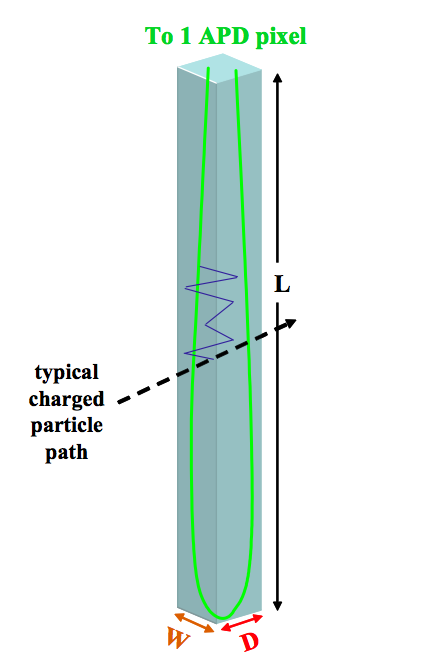
\includegraphics[width=0.4\textwidth]{../../img/det/gen/nova_cell.png}
  \caption{A NOvA cell consisting of an extruded
    PVC tube filled with liquid scintillator and a looped WLS fibre.}
  \label{fig:cell}
\end{figure}


 %module
\begin{figure}
  \centering
  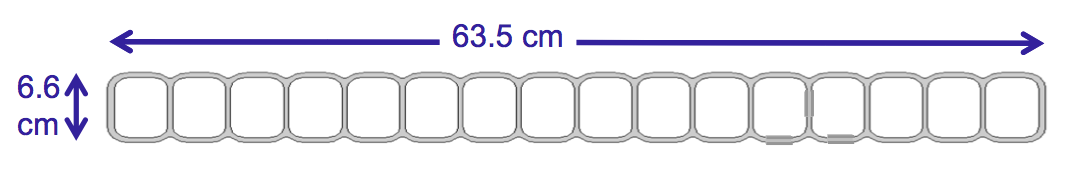
\includegraphics[width=1\textwidth]{../../img/det/gen/extru_cross_section.png}
  \caption{A side on view of a module constructed from 18 cells glued
    together.}
  \label{fig:module}
\end{figure}

%orthogonally stacked planes
\begin{figure}
  \centering
  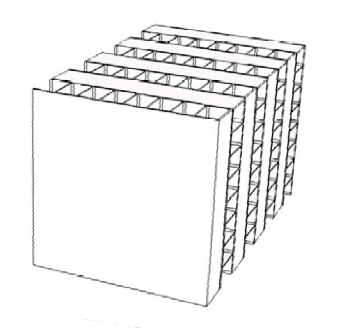
\includegraphics[width=0.5\textwidth]{../../img/det/gen/planes.png}
  \caption{Cut out of a NOvA detector showing the alternating
    orientation of the stacked planes.}
  \label{fig:stackedPlanes}
\end{figure}


% identification of nue and numu from background. use low z, moliere
% radius. distinguish nue from pi0 (see Michaels event displays)


\subsection{Data Aquisition}

Follow from the WLS fibre to APD, to FEB and to DCM.

Explain digitisation via single and multi point readout.


\subsection{The Far Detector}\label{sec:fardet}

Detector on the surface. Overburden of gravel and barrite.

\subsection{The Near Detector}\label{sec:neardet}

Undersground detector. Reduces cosmic ray background.

muon catcher. used to range out muons that would exit otherwise

older APDs. Something to do with the baked/non-baked

faster readout due to higher data rate near the neutrino source
(higher flux)